\documentclass[tikz,border=4pt]{standalone}
\usepackage{amsmath,amssymb}
% Grupo Nostradamus - lenguaje visual TikZ
\definecolor{nostranavy}{HTML}{061426}
\definecolor{nostrateal}{HTML}{078C95}
\definecolor{nostracyan}{HTML}{65DCE5}
\definecolor{nostragold}{HTML}{F5C542}
\newcommand{\sen}{\operatorname{sen}}

\begin{document}
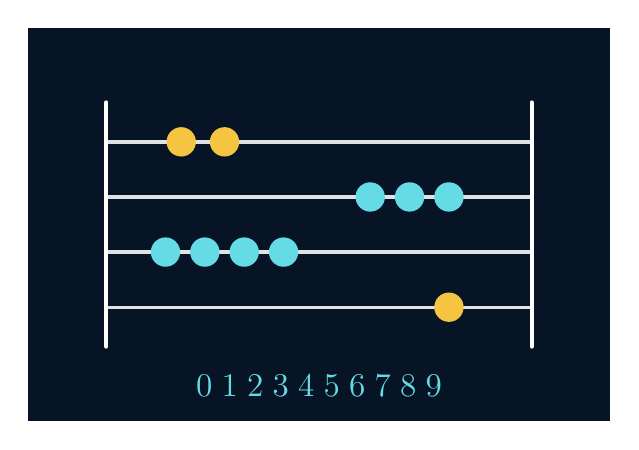
\begin{tikzpicture}[line cap=round,line join=round]
\fill[nostranavy] (-3.7,-2.5) rectangle (3.7,2.5);
\draw[white,line width=1.5pt] (-2.7,-1.55)--(-2.7,1.55) (2.7,-1.55)--(2.7,1.55);
\foreach \y in {-1.05,-.35,.35,1.05}{\draw[white,opacity=.88,line width=1.2pt] (-2.7,\y)--(2.7,\y);}
\foreach \x in {-1.75,-1.20}{\fill[nostragold] (\x,1.05) circle (5.3pt);}
\foreach \x in {.65,1.15,1.65}{\fill[nostracyan] (\x,.35) circle (5.3pt);}
\foreach \x in {-1.95,-1.45,-.95,-.45}{\fill[nostracyan] (\x,-.35) circle (5.3pt);}
\fill[nostragold] (1.65,-1.05) circle (5.3pt);
\node[nostracyan,font=\bfseries\large] at (0,-2.05) {$0\;1\;2\;3\;4\;5\;6\;7\;8\;9$};
\end{tikzpicture}
\end{document}
